%>>>>>>>>>>>>>>>>>>>>>>>>>>>>>>>>>>>>>>>>>>>>>>>>>>>>>>>>>>>>>>>>>>>>>>>>>>>>>>>>>>>>>>>>>>>>>>>>>>>>>>>>>>>>>>>>
\documentclass {beamer}                                                                                         % Crée le document de type Beamer.
\setbeamertemplate {frametitle} [default] [center]                                                              % Permets de centrer les titres des différentes diapositives du projet.
%<<<<<<<<<<<<<<<<<<<<<<<<<<<<<<<<<<<<<<<<<<<<<<<<<<<<<<<<<<<<<<<<<<<<<<<<<<<<<<<<<<<<<<<<<<<<<<<<<<<<<<<<<<<<<<<<
%>>>>>>>>>>>>>>>>>>>>>>>>>>>>>>>>>>>>>>>>>>>>>>>>>>>>>>>>>>>>>>>>>>>>>>>>>>>>>>>>>>>>>>>>>>>>>>>>>>>>>>>>>>>>>>>>
\usepackage [orientation = landscape, size = custom, width = 16, height = 9, scale = 0.5, debug] {beamerposter} % Fais en sorte que les différentes diapositives aient un format d’image 16:9 paysage.
\usepackage [utf8] {inputenc}                                                                                   % Permets d’ajouter des caractères Unicode dans le document latex (autrement, uniquement l’ASCII est supporté).
\usepackage [T1] {fontenc}                                                                                      % Utilisé pour l’encodage des polices d’écriture, empêche d’avoir des caractères inattendus (mal traités après la compilation).
\usepackage {url}                                                                                               % Ajoute la commande \url et permets l’ajout d’adresses e-mail, mais aussi de liens hypertextes, de répertoires et de chemins...
\usepackage {hyperref}                                                                                          % Utilisé pour gérer les commandes de références croisées afin de produire des liens hypertextes dans le document.
%<<<<<<<<<<<<<<<<<<<<<<<<<<<<<<<<<<<<<<<<<<<<<<<<<<<<<<<<<<<<<<<<<<<<<<<<<<<<<<<<<<<<<<<<<<<<<<<<<<<<<<<<<<<<<<<<
%>>>>>>>>>>>>>>>>>>>>>>>>>>>>>>>>>>>>>>>>>>>>>>>>>>>>>>>>>>>>>>>>>>>>>>>>>>>>>>>>>>>>>>>>>>>>>>>>>>>>>>>>>>>>>>>>
\setbeamertemplate {navigation symbols} {}                                                                      % Supprime les éléments de navigations présents de base dans les documents latex.
%<<<<<<<<<<<<<<<<<<<<<<<<<<<<<<<<<<<<<<<<<<<<<<<<<<<<<<<<<<<<<<<<<<<<<<<<<<<<<<<<<<<<<<<<<<<<<<<<<<<<<<<<<<<<<<<<
%>>>>>>>>>>>>>>>>>>>>>>>>>>>>>>>>>>>>>>>>>>>>>>>>>>>>>>>>>>>>>>>>>>>>>>>>>>>>>>>>>>>>>>>>>>>>>>>>>>>>>>>>>>>>>>>>
\AtBeginSection[] {                                                                                             % Permets l’ajout automatique du plan pour chaque nouvelle section.
    \begin {frame}                                                                                              % Crée une nouvelle diapositive dans le projet.
    \frametitle {\insertsectionhead}                                                                            % Définis le titre de la diapositive au titre de la section pour laquelle il crée cette diapositive.
    \tableofcontents [currentsection]                                                                           % Les sections (et leurs sous-sections) autres que celle sur laquelle l’utilisateur est actuellement sont grisées.
    \end {frame}                                                                                                % Indique la fin de la diapositive.
}                                                                                                               % Indique la fin de la fonction.
%<<<<<<<<<<<<<<<<<<<<<<<<<<<<<<<<<<<<<<<<<<<<<<<<<<<<<<<<<<<<<<<<<<<<<<<<<<<<<<<<<<<<<<<<<<<<<<<<<<<<<<<<<<<<<<<<
%>>>>>>>>>>>>>>>>>>>>>>>>>>>>>>>>>>>>>>>>>>>>>>>>>>>>>>>>>>>>>>>>>>>>>>>>>>>>>>>>>>>>>>>>>>>>>>>>>>>>>>>>>>>>>>>>
\begin {document}                                                                                               % Permets de commencer le document latex.
%<<<<<<<<<<<<<<<<<<<<<<<<<<<<<<<<<<<<<<<<<<<<<<<<<<<<<<<<<<<<<<<<<<<<<<<<<<<<<<<<<<<<<<<<<<<<<<<<<<<<<<<<<<<<<<<<
%>>>>>>>>>>>>>>>>>>>>>>>>>>>>>>>>>>>>>>>>>>>>>>>>>>>>>>>>>>>>>>>>>>>>>>>>>>>>>>>>>>>>>>>>>>>>>>>>>>>>>>>>>>>>>>>>
\title {Epitech Project "Indie Studio"}                                                            % Ajout d’un titre pour le document latex (il apparaîtra dans la première diapositive du document).
\author {Amaury Poltavtseef, Antoine Famibelle\\ Aurelien Charpilienne, Camil Lif\\ Nathan Alves, Yoann Mallat} % Ajout d’un auteur pour le document latex (il apparaîtra dans la première diapositive du document).
\date {\today}                                                                                                  % Ajout d’une date actuelle dans le document latex (il apparaîtra dans la première diapositive du document).
\frame {\titlepage}                                                                                             % Permets de donner un titre à la première diapositive.
%<<<<<<<<<<<<<<<<<<<<<<<<<<<<<<<<<<<<<<<<<<<<<<<<<<<<<<<<<<<<<<<<<<<<<<<<<<<<<<<<<<<<<<<<<<<<<<<<<<<<<<<<<<<<<<<<
%>>>>>>>>>>>>>>>>>>>>>>>>>>>>>>>>>>>>>>>>>>>>>>>>>>>>>>>>>>>>>>>>>>>>>>>>>>>>>>>>>>>>>>>>>>>>>>>>>>>>>>>>>>>>>>>>
\section {Bomberman}                                                                                   % Ajout d’une nouvelle section pour structurer le document.
\subsection {What's Bomberman}                                                                  % Ajout d’une nouvelle sous-section pour structurer le document.
\subsection {Neo Bomberman}                                                          % Ajout d’une nouvelle sous-section pour structurer le document.
%<<<<<<<<<<<<<<<<<<<<<<<<<<<<<<<<<<<<<<<<<<<<<<<<<<<<<<<<<<<<<<<<<<<<<<<<<<<<<<<<<<<<<<<<<<<<<<<<<<<<<<<<<<<<<<<<
%>>>>>>>>>>>>>>>>>>>>>>>>>>>>>>>>>>>>>>>>>>>>>>>>>>>>>>>>>>>>>>>>>>>>>>>>>>>>>>>>>>>>>>>>>>>>>>>>>>>>>>>>>>>>>>>>
\frame {\frametitle {What's Bomberman}                                                          % Crée une nouvelle diapositive avec un titre.
\begin {center}                                                                                                 % Définis le début du centrage des éléments.
\normalsize {Everything you need to know about Bomberman :}                                % Affiche un texte en taille normale. 
   \begin {itemize}                                                                                            % Indique le début d’une liste.
        \normalsize {\item {- The player plays a bomber.}}                                                                   % Affiche un texte en taille normale sous forme d’item.
        \par                                                                                                    % Retour à la ligne.
        \normalsize {\item {- The goal is to blow up enemies to win.}}                                                                   % Affiche un texte en taille normale sous forme d’item. 
        \par                                                                                                    % Retour à la ligne. 
       \normalsize {\item {- The player can blow up the walls.}}                                                                   % Affiche un texte en taille normale sous forme d’item.
        \par                                                                                                    % Retour à la ligne.
       \normalsize {\item {- The player can collect bonuses or maluses.}}                                                                   % Affiche un texte en taille normale sous forme d’item.
   \end {itemize}                                                                                              % Indique la fin de la liste.
\end {center}                                                                                                   % Indique la fin du centrage des éléments.
}                                                                                                               % Indique la fin de la diapositive.
%<<<<<<<<<<<<<<<<<<<<<<<<<<<<<<<<<<<<<<<<<<<<<<<<<<<<<<<<<<<<<<<<<<<<<<<<<<<<<<<<<<<<<<<<<<<<<<<<<<<<<<<<<<<<<<<<
%>>>>>>>>>>>>>>>>>>>>>>>>>>>>>>>>>>>>>>>>>>>>>>>>>>>>>>>>>>>>>>>>>>>>>>>>>>>>>>>>>>>>>>>>>>>>>>>>>>>>>>>>>>>>>>>>
\frame {\frametitle {Neo Bomberman}                                                  % Crée une nouvelle diapositive avec un titre.
\begin {center}                                                                                                 % Définis le début du centrage des éléments.

\end {center}                                                                                                   % Indique la fin du centrage des éléments.
\begin {itemize}                                                                                                % Indique le début d'une liste.
    \normalsize {\item {Neo Bomberman dates from 1997.}}                                                                        % Affiche un texte en taille normale sous forme d’item.
    \normalsize {\item {Neo Bomberman is an action-maze arcade video game.}}                     % Affiche un texte en taille normale.
\end {itemize}                                                                                                  % Indique la fin de la liste.
\begin {minipage} [c] {.46\linewidth}                                                                           % Définis le début d’une minipage (permets de mettre les choses les unes à côté des autres) avec l’option centrée et définis la largeur de chaque image à environ la moitié d’une ligne.
    \centering                                                                                                  % Centre le prochain élément.
    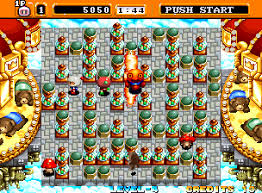
\includegraphics [scale=.50] {content/bomber.jpg}                                                % Ajoute une image dans le document latex en la redimensionnant.
\end {minipage}                                                                                                 % Indique la fin de la minipage.
\hfill                                                                                                          % Fais en sorte de garder un petit espacement entre les images.
\begin {minipage} [c] {.46\linewidth}                                                                           % Définis le début d'une minipage (Permets de mettre les choses les unes à côté des autres) et ajouter l'option centrer et définis la largeur de chaque image à environ la moitié d'une ligne.
    \centering                                                                                                  % Centre le prochain élément.
    
\includegraphics [scale=.50] {content/info.png}                                                         % Ajoute une image dans le document latex en la redimensionnant.
\end {minipage}                                                                                                 % Indique la fin de la minipage.
}                                                                                                               % Indique la fin d’une diapositive.
%<<<<<<<<<<<<<<<<<<<<<<<<<<<<<<<<<<<<<<<<<<<<<<<<<<<<<<<<<<<<<<<<<<<<<<<<<<<<<<<<<<<<<<<<<<<<<<<<<<<<<<<<<<<<<<<<
%>>>>>>>>>>>>>>>>>>>>>>>>>>>>>>>>>>>>>>>>>>>>>>>>>>>>>>>>>>>>>>>>>>>>>>>>>>>>>>>>>>>>>>>>>>>>>>>>>>>>>>>>>>>>>>>>
\section {Project}                                                                                   % Ajout d’une nouvelle section pour structurer le document.
\subsection {Multiplatform}                                                                  % Ajout d’une nouvelle sous-section pour structurer le document.
\subsection {Libraries}                                                          % Ajout d’une nouvelle sous-section pour structurer le document.
\subsection {Main features}                                                          % Ajout d’une nouvelle sous-section pour structurer le document.
\subsection {Messages}                                                                              % Ajout d’une nouvelle sous-section pour structurer le document.
\subsection {Power-Ups}                                                                              % Ajout d’une nouvelle sous-section pour structurer le document.
%<<<<<<<<<<<<<<<<<<<<<<<<<<<<<<<<<<<<<<<<<<<<<<<<<<<<<<<<<<<<<<<<<<<<<<<<<<<<<<<<<<<<<<<<<<<<<<<<<<<<<<<<<<<<<<<<
%>>>>>>>>>>>>>>>>>>>>>>>>>>>>>>>>>>>>>>>>>>>>>>>>>>>>>>>>>>>>>>>>>>>>>>>>>>>>>>>>>>>>>>>>>>>>>>>>>>>>>>>>>>>>>>>>
\frame {\frametitle {Multiplatform}                                                          % Crée une nouvelle diapositive avec un titre.
\begin {center}                                                                                                 % Définis le début du centrage des éléments.
\normalsize {Using CMake 3.11 :}                                % Affiche un texte en taille normale. 
   \begin {itemize}                                                                                            % Indique le début d’une liste.
        \normalsize {\item {Windows (Generation of a Visual Studio .sln solution)}}                                                                   % Affiche un texte en taille normale sous forme d’item.
        \par                                                                                                    % Retour à la ligne.
        \normalsize {\item {Linux (Generation of a Makefile by CMake)}}                                                                   % Affiche un texte en taille normale sous forme d’item. 
   \end {itemize}                                                                                              % Indique la fin de la liste.
\end {center}                                                                                                   % Indique la fin du centrage des éléments.
}                                                                                                               % Indique la fin de la diapositive.
%<<<<<<<<<<<<<<<<<<<<<<<<<<<<<<<<<<<<<<<<<<<<<<<<<<<<<<<<<<<<<<<<<<<<<<<<<<<<<<<<<<<<<<<<<<<<<<<<<<<<<<<<<<<<<<<<
%>>>>>>>>>>>>>>>>>>>>>>>>>>>>>>>>>>>>>>>>>>>>>>>>>>>>>>>>>>>>>>>>>>>>>>>>>>>>>>>>>>>>>>>>>>>>>>>>>>>>>>>>>>>>>>>>
\frame {\frametitle {Libraries}                                                          % Crée une nouvelle diapositive avec un titre.
\begin {center}                                                                                                 % Définis le début du centrage des éléments.
\normalsize {Three libraries used:}                                % Affiche un texte en taille normale. 
   \begin {itemize}                                                                                            % Indique le début d’une liste.
        \normalsize {\item {Irrlicht 1.8.4}}                                                                   % Affiche un texte en taille normale sous forme d’item.
        \par                                                                                                    % Retour à la ligne.
        \normalsize {\item {SFML-audio 2.5}}                                                                   % Affiche un texte en taille normale sous forme d’item. 
        \par                                                                                                    % Retour à la ligne. 
       \normalsize {\item {Boost 1.69}}                                                                   % Affiche un texte en taille normale sous forme d’item.
   \end {itemize}                                                                                              % Indique la fin de la liste.
\end {center}                                                                                                   % Indique la fin du centrage des éléments.
}                                                                                                               % Indique la fin de la diapositive.
%<<<<<<<<<<<<<<<<<<<<<<<<<<<<<<<<<<<<<<<<<<<<<<<<<<<<<<<<<<<<<<<<<<<<<<<<<<<<<<<<<<<<<<<<<<<<<<<<<<<<<<<<<<<<<<<<
%>>>>>>>>>>>>>>>>>>>>>>>>>>>>>>>>>>>>>>>>>>>>>>>>>>>>>>>>>>>>>>>>>>>>>>>>>>>>>>>>>>>>>>>>>>>>>>>>>>>>>>>>>>>>>>>>
\frame {\frametitle {Main features}                                                          % Crée une nouvelle diapositive avec un titre.
\begin {center}                                                                                                 % Définis le début du centrage des éléments.
\normalsize {The main features of the game are: }                                % Affiche un texte en taille normale. 
   \begin {itemize}                                                                                            % Indique le début d’une liste.
        \normalsize {\item {Local multiplayer}}                                                                   % Affiche un texte en taille normale sous forme d’item.
        \par                                                                                                    % Retour à la ligne.
        \normalsize {\item {AI controlled bots}}                                                                   % Affiche un texte en taille normale sous forme d’item. 
        \par                                                                                                    % Retour à la ligne. 
       \normalsize {\item {A main game menu}}                                                                   % Affiche un texte en taille normale sous forme d’item.
        \par                                                                                                    % Retour à la ligne. 
       \normalsize {\item {A backup system}}                                                                   % Affiche un texte en taille normale sous forme d’item.
        \par                                                                                                    % Retour à la ligne. 
       \normalsize {\item {3D graphics seen from above to look like 2D}}                                                                   % Affiche un texte en taille normale sous forme d’item.
        \par                                                                                                    % Retour à la ligne. 
       \normalsize {\item {Map generation}}                                                                   % Affiche un texte en taille normale sous forme d’item.
        \par                                                                                                    % Retour à la ligne. 
       \normalsize {\item {Animations and sounds (bomb, player, background music)}}                                                                   % Affiche un texte en taille normale sous forme d’item.
   \end {itemize}                                                                                              % Indique la fin de la liste.
\end {center}                                                                                                   % Indique la fin du centrage des éléments.
}                                                                                                               % Indique la fin de la diapositive.
%<<<<<<<<<<<<<<<<<<<<<<<<<<<<<<<<<<<<<<<<<<<<<<<<<<<<<<<<<<<<<<<<<<<<<<<<<<<<<<<<<<<<<<<<<<<<<<<<<<<<<<<<<<<<<<<<
%>>>>>>>>>>>>>>>>>>>>>>>>>>>>>>>>>>>>>>>>>>>>>>>>>>>>>>>>>>>>>>>>>>>>>>>>>>>>>>>>>>>>>>>>>>>>>>>>>>>>>>>>>>>>>>>>
\frame {\frametitle {Power-Ups}                                                          % Crée une nouvelle diapositive avec un titre.
\begin {center}                                                                                                 % Définis le début du centrage des éléments.
\normalsize {List of the Power-Ups:}                                % Affiche un texte en taille normale. 
   \begin {itemize}                                                                                            % Indique le début d’une liste.
        \normalsize {\item {Extra Bomb}}                                                                   % Affiche un texte en taille normale sous forme d’item.
        \par                                                                                                    % Retour à la ligne.
        \normalsize {\item {Acceleration}}                                                                   % Affiche un texte en taille normale sous forme d’item. 
        \par                                                                                                    % Retour à la ligne. 
       \normalsize {\item {Increase in bomb strength}}                                                                   % Affiche un texte en taille normale sous forme d’item.
        \par                                                                                                    % Retour à la ligne. 
       \normalsize {\item {Going through a wall}}                                                                   % Affiche un texte en taille normale sous forme d’item.
   \end {itemize}                                                                                              % Indique la fin de la liste.
\end {center}                                                                                                   % Indique la fin du centrage des éléments.
}                                                                                                               % Indique la fin de la diapositive.
%<<<<<<<<<<<<<<<<<<<<<<<<<<<<<<<<<<<<<<<<<<<<<<<<<<<<<<<<<<<<<<<<<<<<<<<<<<<<<<<<<<<<<<<<<<<<<<<<<<<<<<<<<<<<<<<<
%>>>>>>>>>>>>>>>>>>>>>>>>>>>>>>>>>>>>>>>>>>>>>>>>>>>>>>>>>>>>>>>>>>>>>>>>>>>>>>>>>>>>>>>>>>>>>>>>>>>>>>>>>>>>>>>>
\end {document}                                                                                                 % Permets de terminer le document latex.
%<<<<<<<<<<<<<<<<<<<<<<<<<<<<<<<<<<<<<<<<<<<<<<<<<<<<<<<<<<<<<<<<<<<<<<<<<<<<<<<<<<<<<<<<<<<<<<<<<<<<<<<<<<<<<<<<
